\tikzstyle{startstop} = [rectangle, rounded corners, minimum width=10cm, minimum height=1.5cm,text centered, draw=black, fill=green!20]
\begin{center}
	\begin{tikzpicture}
		\node (start) [startstop] {\bfseries \text{ÔN TẬP BÀI 1 VÀ BÀI 2}};
	\end{tikzpicture}
\end{center}
\setcounter{section}{0}
\section{Câu trắc nghiệm nhiều phương án lựa chọn}
\Opensolutionfile{ans}[ans/G12BT1+2TN]
% ===================================================================
\begin{ex}
	Với mô hình động học phân tử, sự khác biệt về cấu trúc của chất rắn, chất lỏng, chất khí là do sự khác biệt về
	\choice
	{thành phần các phân tử cấu tạo của mỗi chất}
	{\True độ lớn lực tương tác giữa các phân tử trong mỗi chất}
	{số lượng phân tử cấu tạo nên mỗi chất}
	{kích thước của các phân tử cấu tạo mỗi chất}
	\loigiai{}
\end{ex}
% ===================================================================
\begin{ex}
Khi nói về khoảng cách trung bình giữa các phân tử trong chất rắn, chất lỏng, chất khí. Kết luận nào sau đây là \textbf{đúng}?	
	\choice
	{Khoảng cách giữa các phân tử trong chất lỏng xa hơn so với các phân tử trong chất khí}
	{Khoảng cách giữa các phân tử trong chất rắn xa hơn so với các phân tử trong chất lỏng}
	{\True Khoảng cách giữa các phân tử trong chất lỏng gần hơn so với các phân tử trong chất khí}
	{Khoảng cách giữa các phân tử trong chất lỏng xa hơn so với các phân tử trong chất khí}
	\loigiai{}
\end{ex}
% ===================================================================
\begin{ex}
	Câu nào dưới đây nói về đặc tính của chất rắn kết tinh là \textbf{không đúng}?
	\choice
	{Các nguyên tử, phân tử liên kết chặt với nhau và sắp xếp theo một trật tự hình học xác định}
	{\True Không có nhiệt độ nóng chảy xác định}
	{Có cấu trúc tinh thể}
	{Có nhiệt độ nóng chảy xác định}
	\loigiai{}
\end{ex}
% ===================================================================
\begin{ex}
	Chất rắn nào dưới đây thuộc loại chất rắn vô định hình?
	\choice
	{Muối ăn}
	{Nhựa đường}
	{Kim loại}
	{Kim cương}
	\loigiai{}
\end{ex}
% ===================================================================
\begin{ex}
	Chất lỏng không có hình dạng xác định vì các phân tử chất lỏng
	\choice
	{dao động tại các vị trí cân bằng xác định}
	{có thể chuyển động phân tán ra xa nhau}
	{\True dao động quanh các vị trí cân bằng có thể dịch chuyển được}
	{có thể chuyển động tự do}
	\loigiai{}
\end{ex}
% ===================================================================
\begin{ex}
Chất khí dễ bị nén hơn so với chất rắn và chất lỏng vì	
	\choice
	{lực tương tác giữa các phân tử trong chất khí lớn hơn so với lực tương tác giữa các phân tử trong chất rắn và chất lỏng}
	{\True khoảng cách giữa các phân tử trong chất khí lớn hơn so với khoảng cách giữa các phân tử trong chất rắn và chất lỏng}
	{các phân tử trong chất khí ít chuyển động hơn so với các phân tử trong chất rắn và chất lỏng}
	{các phân tử trong chất khí có kích thước nhỏ hơn so với các phân tử trong chất rắn và chất lỏng}
	\loigiai{}
\end{ex}
% ===================================================================
\begin{ex}
Khi nói về quá trình nóng chảy và đông đặc là đang nói về quá trình chuyển thể giữa	
	\choice
	{chất rắn và chất khí}
	{chất khí và chất lỏng}
	{\True chất rắn và chất lỏng}
	{các chất bất kì}
	\loigiai{}
\end{ex}
% ===================================================================
\begin{ex}
	Quá trình chuyển từ thể khí sang thể rắn của các chất được gọi là
	\choice
	{\True sự ngưng kết}
	{thăng hoa}
	{sự đông đặc}
	{sự ngưng tụ}
	\loigiai{}
\end{ex}
% ===================================================================
\begin{ex}
	Khi chất rắn kết tinh được nung nóng. Kết luận nào sau đây là \textbf{đúng}?
	\choice
	{các phân tử vẫn dao động với biên độ không đổi, khoảng cách giữa các phân tử không đổi}
	{\True các phân tử dao động với biên độ tăng lên, khoảng cách giữa các phân tử tăng lên}
	{các phân tử dao động với biên độ không đổi, khoảng cách giữa các phân tử tăng lên}
	{các phân tử dao động với biên độ tăng lên, khoảng cách giữa các phân tử không đổi}
	\loigiai{}
\end{ex}
% ===================================================================
\begin{ex}
	Sự nóng chảy của chất rắn kết tinh bắt đầu xảy ra khi
	\choice
	{một số phân tử dao động mạnh hơn các phân tử xung quanh}
	{một số phân tử va chạm với các phân tử xung quanh}
	{một số phân tử dao động mạnh lên và truyền năng lượng dao động cho các phân tử khác}
	{\True một số phân tử thắng được lực liên kết với các phân tử xung quanh và thoát khỏi liên kết với chúng}
	\loigiai{}
\end{ex}
% ===================================================================
\begin{ex}
Trong quá trình chất rắn kết tinh đang nóng chảy nhiệt độ của nó không tăng thêm là do
	\choice
	{phần nhiệt nhận thêm cân bằng với phần nhiệt toả ra môi trường bên ngoài}
	{phần nhiệt lượng nhận thêm đã chuyển thành động năng của các phân tử}
	{\True phần nhiệt lượng nhận thêm đã chuyển thành năng lượng để tiếp tục phá vỡ liên kết của mạng tinh thể}
	{phần nhiệt lượng nhận thêm đã chuyển thành thế năng của các phân tử}
	\loigiai{}
\end{ex}
% ===================================================================
\begin{ex}
	Khi cho một cục nước đá vào nước ở nhiệt độ phòng thì kết luận nào sau đây là \textbf{đúng}?
	\choice
	{Nhiệt độ của nước trong cốc từ từ tăng lên}
	{Nước trong cốc sẽ nhận nhiệt lượng từ cục nước đá}
	{\True Nhiệt lượng được truyền từ nước trong cốc cho cục nước đá}
	{Quá trình truyền nhiệt kết thúc khi cục nước đá tan hết.}
	\loigiai{}
\end{ex}
% ===================================================================
\begin{ex}
	Có ba vật A, B, C có các nhiệt độ lần lượt là $t_\text{A}$, $t_\text{B}$, $t_\text{C}$. Cho vật A tiếp xúc với vật B đến khi cân bằng nhiệt, ngay sau đó lại cho vật A tiếp xúc với vật C đến khi cân bằng nhiệt thì nhiệt độ của vật A lúc này bằng với nhiệt độ của nó lúc ban đầu khi chưa tiếp xúc với các vật khác. Kết luận nào sau đây là \textbf{đúng}?
	\choice
	{Vật B đóng vai trò truyền nhiệt lượng khi tiếp xúc với vật A}
	{Vật C đóng vai trò nhận nhiệt lượng khi tiếp xúc với vật A}
	{Nhiệt độ của vật B thấp hơn nhiệt độ của vật C}
	{\True Tổng nhiệt lượng mà vật A nhận được bằng tổng nhiệt lượng mà nó truyền cho vật khác}
	\loigiai{}
\end{ex}
% ===================================================================
\begin{ex}
	Gọi $t_1$, $t_2$ lần lượt là nhiệt độ điểm đóng băng và nhiệt độ sôi của nước tinh khiết ở điều kiện áp suất tiêu chuẩn. Trong thang nhiệt độ Celsius, mỗi độ chia $\left(\SI{1}{\celsius}\right)$ có độ lớn bằng
	\choice
	{$100\left(t_2-t_1\right)$}
	{$100\left(t_1-t_2\right)$}
	{\True $\dfrac{1}{100}\left(t_2-t_1\right)$}
	{$\dfrac{1}{273,15}\left(t_2-t_1\right)$}
	\loigiai{}
\end{ex}
% ===================================================================
\begin{ex}
Nhiệt độ không tuyệt đối là nhiệt độ mà tại đó tất cả các chất có	
	\choice
	{động năng chuyển động nhiệt của các nguyên tử hoặc phân tử bằng không và thế năng của chúng là cực đại}
	{động năng chuyển động nhiệt của các nguyên tử hoặc phân tử là cực đại và thế năng của chúng là tối thiểu}
	{\True động năng chuyển động nhiệt của các nguyên tử hoặc phân tử bằng không và thế năng của chúng là tối thiểu}
	{động năng chuyển động nhiệt của các nguyên tử hoặc phân tử và thế năng của chúng là cực đại}
	\loigiai{}
\end{ex}
% ===================================================================
\begin{ex}
Gọi $\Delta t$ và $\Delta T$ lần lượt  là độ lớn một độ chia trên thang đo nhiệt độ Celsius và thang đo nhiệt độ Kelvin. Hệ thức nào sau đây là \textbf{đúng}?
	\choice
	{$\Delta t=\dfrac{1}{273}\Delta T$}
	{$\Delta t=273\Delta T$}
	{$\Delta T=\dfrac{1}{100}\Delta t$}
	{\True $\Delta T =\Delta t$}
	\loigiai{}
\end{ex}
% ===================================================================
\begin{ex}
Kết luận nào sau đây về nhiệt độ của một vật là \textbf{đúng}?	
	\choice
	{Nhiệt độ của một vật bất kì luôn có giá trị lớn hơn $\SI{0}{\celsius}$}
	{Nhiệt độ của một vật bất kì tỉ lệ thuận với khối lượng của nó}
	{Nhiệt độ của một vật bất kì phụ thuộc vào khoảng cách giữa các phân tử trong mạng tinh thể}
	{\True Nhiệt độ của một vật bất kì không thể nhỏ hơn $\SI{0}{\kelvin}$}
	\loigiai{}
\end{ex}
% ===================================================================
\begin{ex}
Một thang nhiệt độ Z có nhiệt độ đóng băng của nước là $-\SI{12}{\degree Z}$ và khoảng cách mỗi độ chia trong thang đo nhiệt độ Z có độ lớn bằng $\SI{0.8}{}$	lần khoảng cách một độ chia trong thang đo nhiệt độ Kelvin. Nhiệt độ sôi của nước trong thang nhiệt độ Z là
	\choice
	{\True $\SI{113}{\degree Z}$}
	{$\SI{137}{\degree Z}$}
	{$\SI{68}{\degree Z}$}
	{$\SI{92}{\degree Z}$}
	\loigiai{$\Delta t_Z=0,8\Delta T\Rightarrow \left(t_Z+12\right)=0,8\cdot 100\Rightarrow t_Z=\SI{113}{\degree Z}$.}
\end{ex}
% ===================================================================
\begin{ex}
Một thang đo nhiệt độ Y, trong đó nhiệt độ nước đá đang tan là $-\SI{25}{\degree Y}$ và nhiệt độ sôi của nước là $\SI{85}{\degree Y}$. Nhiệt độ $\SI{70}{\degree Y}$ sẽ gần đúng tương ứng với nhiệt độ trong thang nhiệt độ Kelvin là	
	\choice
	{\True $\SI{360}{\kelvin}$}
	{$\SI{377}{\kelvin}$}
	{$\SI{350}{\kelvin}$}
	{$\SI{366}{\kelvin}$}
	\loigiai{
$\dfrac{t_Y+25}{85+25}=\dfrac{T-273}{100}$.	
}
% ===================================================================
\begin{ex}
Có hai thang đo nhiệt độ X và Y liên hệ với nhau theo công thức $T_\text{X}=\dfrac{3}{4}T_\text{Y}+20$. Độ biến thiên nhiệt độ $\SI{30}{\degree X}$ trong thang nhiệt X sẽ tương ứng với một độ biến thiên trong thang nhiệt Y là	
	\choice
	{$\SI{66.6}{\degree Y}$}
	{\True $\SI{40}{\degree Y}$}
	{$\SI{60}{\degree Y}$}
	{$\SI{86.6}{\degree Y}$}
	\loigiai{}
\end{ex}
\end{ex}
\Closesolutionfile{ans}
\section{Trắc nghiệm đúng/sai}
\setcounter{ex}{0}
\Opensolutionfile{ans}[ans/G12B1+2TF]
% ===================================================================
\begin{ex}
	Khi nung nóng một chất rắn kết tinh ở áp suất tiêu chuẩn, nhiệt độ của chất rắn tăng lên đến một giá trị nào đó thì chất rắn bắt đầu chuyển sang thể lỏng. Quá trình này được gọi là quá trình nóng chảy.
	\choiceTF[t]
	{\True Nhiệt độ mà chất rắn kết tinh bắt đầu nóng chảy gọi là nhiệt độ nóng chảy}
	{\True Trong quá trình nung nóng, các phân tử của chất rắn sẽ dao động mạnh làm tăng khoảng cách giữa chúng}
	{Nhiệt độ của chất rắn kết tinh tăng liên tục trong quá trình nung nóng đến khi nó nóng chảy hoàn toàn}
	{\True Sau khi chuyển sang thể lỏng, nếu ngừng cung cấp nhiệt lượng thì chất lỏng sẽ bắt đầu quá trình đông đặc}
	\loigiai{}
\end{ex}
% ===================================================================
\begin{ex}
\immini{
Máy thuỷ lực là một thiết bị quan trọng trong ngành xây dựng, kỹ thuật ô tô, \dots. Bên trong máy thuỷ lực người ta dùng một chất lỏng (dầu thuỷ lực). Khi ta tác dụng một lực $f$ lên piston nhỏ có diện tích $s$ lực này gây ra áp suất $p=f/s$ và được truyền nguyên vẹn đến piston lớn có diện tích $S$ và gây ra lực nâng $F$.	
}
{
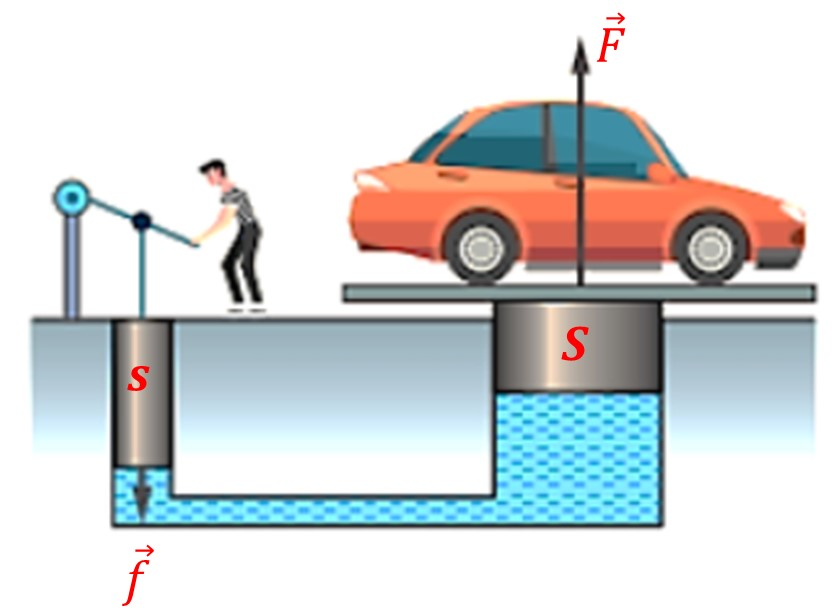
\includegraphics[width=0.6\linewidth]{figs/G12-BT1+2-1}
}
	\choiceTF[t]
	{Có thể thay thế chất lỏng trong máy thuỷ lực bằng chất khí}
	{Người ta sử dụng dầu thuỷ lực vì dầu thuỷ lực có đặc tính rất khó bị nén}
	{\True Nếu người ta nén với lực $f$ rất lón, các phân tử chất lỏng trong máy thuỷ lực càng bị nén chặt và có thể chuyển sang thể rắn}
	{Giả sử piston lớn có diện tích gấp 50 lần piston nhỏ. Khi đó, nếu muốn nâng một xe có khối lượng $\SI{1500}{\kilogram}$ thì cần tác dụng lên piston nhỏ một lực $\SI{30}{\newton}$}
	\loigiai{
\begin{itemchoice}
	\itemch Sai. Vì chất khí dễ bị nén nên máy không hoạt động được.
	\itemch Đúng.
	\itemch Sai. Chất lỏng không thể chuyển thành thể rắn khi chỉ bị nén.
	\itemch Sai. $p=\dfrac{f}{s}=\dfrac{F}{S}\Rightarrow f=\dfrac{Fs}{S}=\SI{300}{\newton}$.
	
	\end{itemchoice}	
}
\end{ex}
% ===================================================================
\begin{ex}

\immini{
Để tạo ra các loại rượu truyền thống đặc trưng của Việt Nam, các cơ sở sản xuất rượu đã thực hiện nhiều công đoạn. Trong các công đoạn đó có một công đoạn rất quan trọng là quá trình chưng cất rượu. Quá	trình chưng cất được thể hiện đơn giản bằng sơ đồ hình bên.
}
{
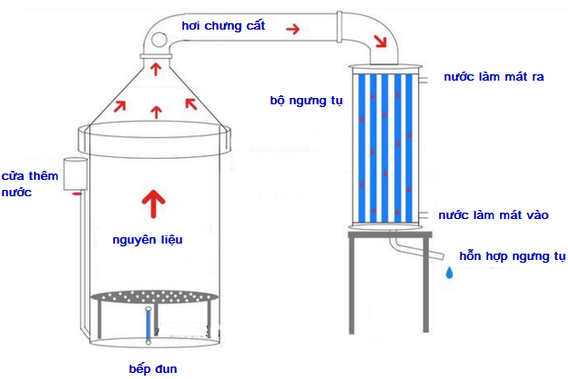
\includegraphics[width=0.7\linewidth]{figs/G12-BT1+2-2}
}
	\choiceTF[t]
	{\True Ở bồn A hỗn hợp nguyên liệu lỏng được cung cấp nhiệt lượng để tạo hơi rượu}
	{Rượu có nhiệt độ sôi cao hơn nước nên rượu hoá hơi trước}
	{Nước làm mát ở bồn B có tác dụng cung cấp nhiệt lượng cho quá trình ngưng tụ của hơi rượu}
	{\True Thực ra trong hỗn hợp hơi vừa có hơi rượu vừa có hơi nước}
	\loigiai{}
\end{ex}
% ===================================================================
\begin{ex}
	\immini{
Máy làm lạnh là một thiết bị khá quen thuộc trong đời sống hằng ngày. Nguyên tắc hoạt động của máy dựa trên nguyên tắc chuyển thể của môi chất gas bên trong máy. Sự trao đổi nhiệt với môi trường diễn ra ở giàn nóng và giàn lạnh của máy.	
}
{
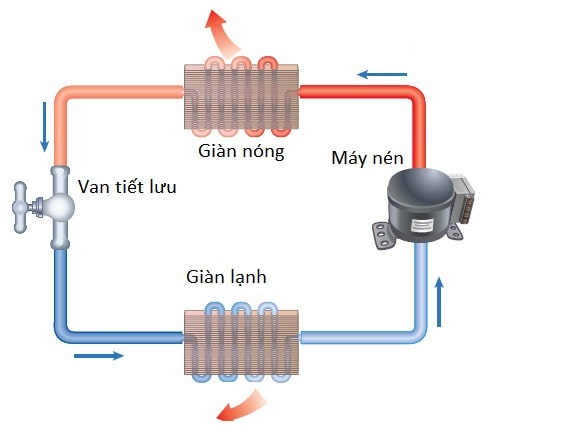
\includegraphics[width=0.65\linewidth]{figs/G12-BT1+2-3}
}
	\choiceTF[t]
	{\True Tại giàn nóng, gas có sự chuyển thể từ dạng khí sang lỏng}
	{\True Tại giàn lạnh, gas có sự chuyển thể từ dạng lỏng sang khí}
	{Tại giàn nóng, gas đã thu nhiệt từ môi trường}
	{Tại giàn lạnh, gas đã toả nhiệt ra môi trường}
	\loigiai{}
\end{ex}
% ===================================================================
\begin{ex}
	Hình bên là đồ thị phác hoạ sự thay đổi nhiệt độ theo thời gian trong quá trình chuyển thể từ rắn sang lỏng của chất rắn kết tinh và chất rắn vô định hình.
\begin{center}
	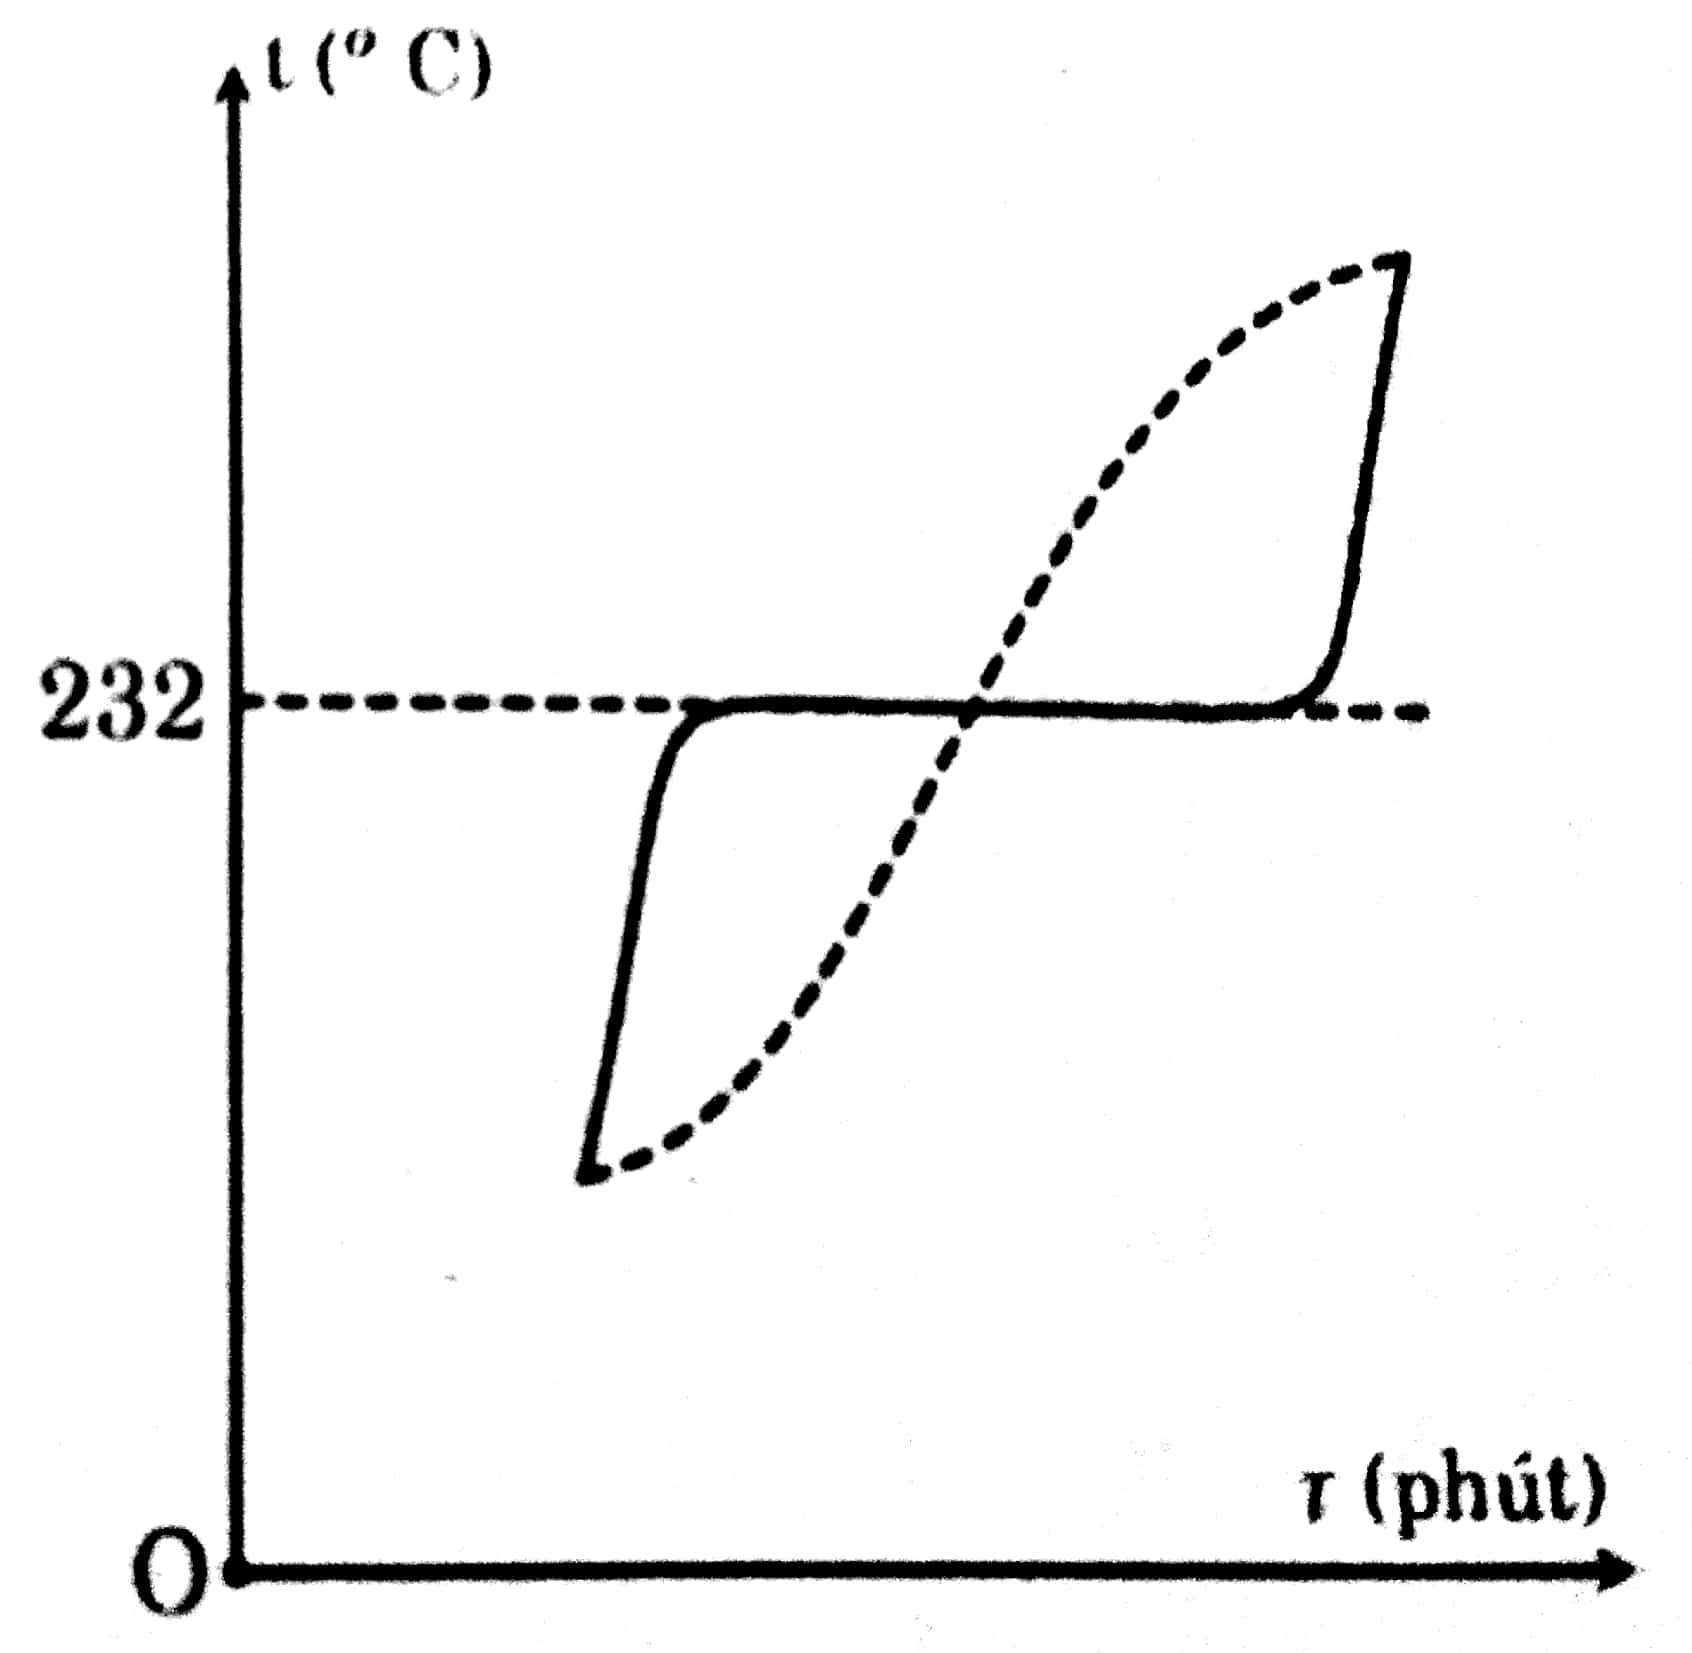
\includegraphics[width=0.3\linewidth]{figs/G12-BT1+2-4}
\end{center}
	\choiceTF[t]
	{Đường nét liền mô tả quá trình chuyển thể của chất rắn vô định hình}
	{Đường nét đứt mô tả quá trình chuyển thể của chất rắn kết tinh}
	{\True Nhiệt độ nóng chảy của chất rắn kết tinh là $\SI{232}{\celsius}$}
	{Chất rắn vô định hình có nhiệt độ nóng chảy cao hơn chất rắn kết tinh}
	\loigiai{}
\end{ex}

% ===================================================================
\begin{ex}
Có hai chai nước lạnh A và B giống nhau (cùng nhiệt độ, cùng thể tích).
\begin{enumerate}[label=\bfseries\itshape Lần \arabic*:, leftmargin=1.5cm]
	\item Nhúng chai A vào chậu nước, nhiệt độ nước trong chậu giảm xuống. Đến khi hệ cân bằng nhiệt thì lấy chai A ra khỏi chậu.
	\item Nhúng chai nước B vào chậu nước, nhiệt độ nước trong chậu tiếp tục giảm xuống đến khi cân bằng nhiệt thì lấy chai nước B ra khỏi chậu.
\end{enumerate}
	\choiceTF[t]
	{\True Nhiệt độ của chai nước A sau khi lấy ra khỏi chậu cao hơn nhiệt độ chai nước B}
	{Nhiệt lượng của chậu nước truyền cho hai chai nước là như nhau}
	{\True Độ giảm nhiệt độ của chậu nước trong lần nhúng thứ nhất nhiều hơn lần nhúng thứ hai}
	{Tổng độ tăng nhiệt độ của hai chai nước bằng tổng độ giảm nhiệt độ của chậu nước trong hai lần nhúng}
	\loigiai{}
\end{ex}
% ===================================================================
\begin{ex}
	Hình bên mô tả mối liên hệ giữa hai thang đo nhiệt độ Kelvin và Fahrenheit ở điều kiện áp suất tiêu chuẩn.
	\begin{center}
		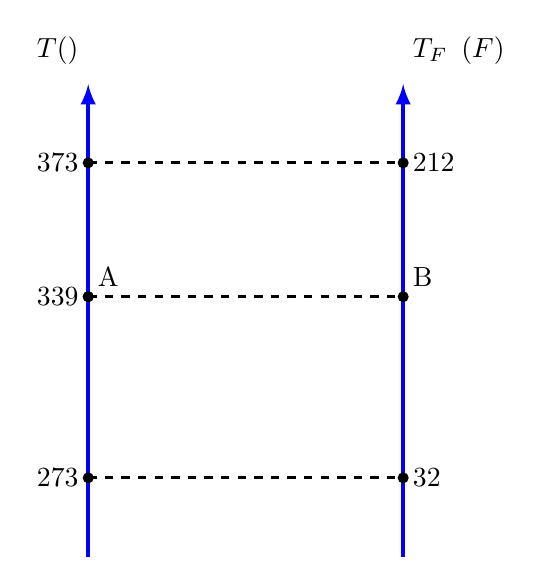
\begin{tikzpicture}
			\draw[line width=1.5pt, blue, -latex] (0,0)--(0,6);
			\draw[line width=1.5pt, blue, -latex] (4,0)--(4,6);
			\draw[line width=1pt, dashed] (0,1)--(4,1);
			\draw[line width=1pt, dashed] (0,5)--(4,5);
			\draw[line width=1pt, dashed] (0,3.3)--(4,3.3);
			\fill   (0,1) circle[radius=2pt]  node [left] {$273$};
			\fill   (4,1) circle[radius=2pt]  node [right] {$32$};
			\fill   (0,5) circle[radius=2pt]  node [left] {$373$};
			\fill   (4,5) circle[radius=2pt]  node [right] {$212$};
			\fill   (0,3.3) circle[radius=2pt]  node [left] {$339$};
			\fill   (0,3.3) circle[radius=2pt]  node [above right] {A};
			\fill   (4,3.3) circle[radius=2pt]  node [above right] {B};
			\node[label={[above left]90:$\xsi{T}{\left(\kelvin\right)}$}] at (0,6){};
			\node[label={[above right]90:$T_F\ \left(\si{\degree F}\right)$}] at (4,6){};
		\end{tikzpicture}
	\end{center}
	\choiceTF[t]
	{Mỗi độ chia trong thang đo nhiệt độ Fahrenheit có độ lớn bằng 1,8 lần mỗi độ chia trong thang đo nhiệt độ Kelvin}
	{\True Độ biến thiên nhiệt độ là $\SI{100}{\kelvin}$ trên thang đo nhiệt độ Kelvin sẽ tương ứng với độ biến thiên $\SI{180}{\degree F}$ trên thang đo nhiệt độ Fahrenheit}
	{\True Tại điểm B trên hình theo thang nhiệt độ Fahrenheit có nhiệt độ là $\SI{150.8}{\degree F}$}
	{\True Tại nhiệt độ $\SI{574.25}{}$ độ thì giá trị trên hai thang đo là bằng nhau}
	\loigiai{}
\end{ex}
% ===================================================================
\begin{ex}
Người ta dùng lò nấu chảy kim loại để nấu chảy sắt. Hình bên là đồ thị ghi lại sự thay đổi nhiệt độ của sắt theo thời gian.
\begin{center}
	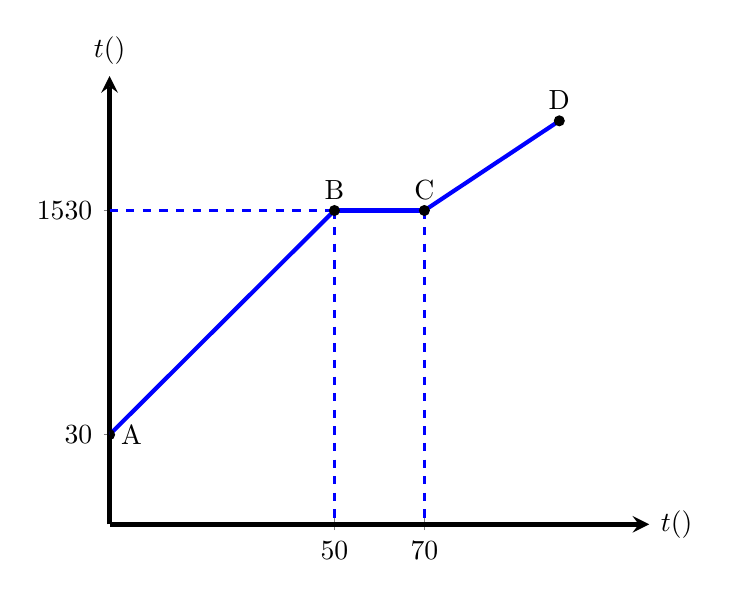
\begin{tikzpicture}  
		\begin{axis}[  ultra thick,
			xmin=0,  
			xmax=12,  
			xtick={0,5, 7},
			ytick={0,2,7},
%			minor x tick num=3,
%			minor y tick num=1,
			ymin=0,  
			ymax=10, 
			xticklabels={0,50,70},
			yticklabels={0,30,1530},
			samples=300,
			axis lines=middle, 
%			grid style={step=1,line width=0.4pt, color=gray!20!white},
%			grid=both,
%			major grid style={line width=0.8pt,gray!60!white},
			xlabel=$\xsi{t}{\left(\minute\right)}$, 
			ylabel=$\xsi{t}{\left(\si{\celsius}\right)}$, 
			every axis y label/.style={at=(current axis.above origin),anchor=south},  
			every axis x label/.style={at=(current axis.right of origin),anchor=west}]  
			\draw[line width=1.5pt, blue] (axis cs: 0,2)--(axis cs: 5,7);
			\draw[line width=1.5pt, blue] (axis cs: 5,7)--(axis cs: 7,7);
			\draw[line width=1.5pt, blue] (axis cs: 7,7)--(axis cs: 10,9);
			\draw[line width=1pt, dashed, blue] (axis cs: 5,7)--(axis cs: 5,0);
			\draw[line width=1pt, dashed, blue] (axis cs: 7,7)--(axis cs: 7,0);
			\draw[line width=1pt, dashed, blue] (axis cs: 0,7)--(axis cs: 5,7);
			\fill   (axis cs: 0,2) circle[radius=2pt]  node [right] {A};
			\fill   (axis cs: 5,7) circle[radius=2pt]  node [above] {B};
			\fill   (axis cs: 7,7) circle[radius=2pt]  node [above] {C};
			\fill   (axis cs: 10,9) circle[radius=2pt]  node [above] {D};
		\end{axis}  
	\end{tikzpicture}
\end{center}	
	\choiceTF[t]
	{\True Kể từ thời điểm ban đầu đến phút thứ 50, sắt vẫn ở thể rắn}
	{\True Nhiệt độ nóng chảy của sắt là $\SI{1530}{\celsius}$}
	{\True Từ phút thứ 50 đến phút thứ 70 là giai đoạn chuyển từ thể rắn sang thể lỏng}
	{Đoạn CD trên đồ thị thể hiện quá trình sôi của sắt}
	\loigiai{}
\end{ex}
% ===================================================================
\begin{ex}
	Giả sử có một thang đo nhiệt độ Z với nhiệt độ điểm đóng băng của nước tinh khiết là $-\SI{10}{\degree Z}$ và nhiệt độ sôi là $\SI{140}{\degree Z}$, biết rằng trong thang nhiệt độ Celsius nhiệt độ các điểm trên là $\SI{0}{\celsius}$ và $\SI{100}{\celsius}$ (các nhiệt độ đều được ghi nhận ở điều kiện áp suất tiêu chuẩn)
	\choiceTF[t]
	{\True Khoảng cách mỗi độ chia trong hai thang đo nhiệt độ là khác nhau}
	{Nếu độ biến thiên nhiệt độ là $\SI{10}{\celsius}$ trong thang nhiệt độ Celsius tương ứng với độ biến thiên $\SI{25}{\degree Z}$ trong thang nhiệt độ Z}
	{\True Nhiệt độ giữa hai thang đo nhiệt độ liên hệ với nhau $t=\dfrac{2}{3}T_\text{Z}+\dfrac{20}{3}$}
	{Nhiệt độ cơ thể người là $\SI{37}{\celsius}$ theo thang nhiệt Celsius thì tương ứng với nhiệt độ $\SI{55.5}{\degree Z}$}
	\loigiai{}
\end{ex}
\Closesolutionfile{ans}